% THIS DOCUMENT IS TAILORED TO REQUIREMENTS FOR SCIENTIFIC COMPUTING.  IT SHOULDN'T
% BE USED FOR NON-SCIENTIFIC COMPUTING PROJECTS
\documentclass[12pt]{article}

\usepackage{amsmath, mathtools}
\usepackage{amsfonts}
\usepackage{amssymb}
\usepackage{graphicx}
\usepackage{cite}
\usepackage{colortbl}
\usepackage{xr}
\usepackage{hyperref}
\usepackage{longtable}
\usepackage{xfrac}
\usepackage{tabularx}
\usepackage{float}
\usepackage{siunitx}
\usepackage{booktabs}
\usepackage{caption}
\usepackage{pdflscape}
\usepackage{afterpage}
\usepackage{datetime2}
\usepackage{pdflscape}

\usepackage[round]{natbib}

%\usepackage{refcheck}

\hypersetup{
    bookmarks=true,         % show bookmarks bar?
      colorlinks=true,       % false: boxed links; true: colored links
    linkcolor=red,          % color of internal links (change box color with linkbordercolor)
    citecolor=green,        % color of links to bibliography
    filecolor=magenta,      % color of file links
    urlcolor=cyan           % color of external links
}

%% Comments

\usepackage{color}

\newif\ifcomments\commentstrue %displays comments
%\newif\ifcomments\commentsfalse %so that comments do not display

\ifcomments
\newcommand{\authornote}[3]{\textcolor{#1}{[#3 ---#2]}}
\newcommand{\todo}[1]{\textcolor{red}{[TODO: #1]}}
\else
\newcommand{\authornote}[3]{}
\newcommand{\todo}[1]{}
\fi

\newcommand{\wss}[1]{\authornote{blue}{SS}{#1}} 
\newcommand{\plt}[1]{\authornote{magenta}{TPLT}{#1}} %For explanation of the template
\newcommand{\an}[1]{\authornote{cyan}{Author}{#1}}

%% Common Parts

\newcommand{\progname}{ProgName} % PUT YOUR PROGRAM NAME HERE
\newcommand{\authname}{Team \#, Team Name
\\ Student 1 name
\\ Student 2 name
\\ Student 3 name
\\ Student 4 name} % AUTHOR NAMES                  

\usepackage{hyperref}
    \hypersetup{colorlinks=true, linkcolor=blue, citecolor=blue, filecolor=blue,
                urlcolor=blue, unicode=false}
    \urlstyle{same}
                                


% For easy change of table widths
\newcommand{\colZwidth}{1.0\textwidth}
\newcommand{\colAwidth}{0.13\textwidth}
\newcommand{\colBwidth}{0.82\textwidth}
\newcommand{\colCwidth}{0.1\textwidth}
\newcommand{\colDwidth}{0.05\textwidth}
\newcommand{\colEwidth}{0.8\textwidth}
\newcommand{\colFwidth}{0.17\textwidth}
\newcommand{\colGwidth}{0.5\textwidth}
\newcommand{\colHwidth}{0.28\textwidth}

% Used so that cross-references have a meaningful prefix
\newcounter{defnum} %Definition Number
\newcommand{\dthedefnum}{GD\thedefnum}
\newcommand{\dref}[1]{GD\ref{#1}}
\newcounter{datadefnum} %Datadefinition Number
\newcommand{\ddthedatadefnum}{DD\thedatadefnum}
\newcommand{\ddref}[1]{DD\ref{#1}}
\newcounter{theorynum} %Theory Number
\newcommand{\tthetheorynum}{TM\thetheorynum}
\newcommand{\tref}[1]{TM\ref{#1}}
\newcounter{tablenum} %Table Number
\newcommand{\tbthetablenum}{TB\thetablenum}
\newcommand{\tbref}[1]{TB\ref{#1}}
\newcounter{assumpnum} %Assumption Number
\newcommand{\atheassumpnum}{A\theassumpnum}
\newcommand{\aref}[1]{A\ref{#1}}
\newcounter{goalnum} %Goal Number
\newcommand{\gthegoalnum}{GS\thegoalnum}
\newcommand{\gsref}[1]{GS\ref{#1}}
\newcounter{instnum} %Instance Number
\newcommand{\itheinstnum}{IM\theinstnum}
\newcommand{\iref}[1]{IM\ref{#1}}
\newcounter{reqnum} %Requirement Number
\newcommand{\rthereqnum}{R\thereqnum}
\newcommand{\rref}[1]{R\ref{#1}}
\newcounter{nfrnum} %NFR Number
\newcommand{\rthenfrnum}{NFR\thenfrnum}
\newcommand{\nfrref}[1]{NFR\ref{#1}}
\newcounter{lcnum} %Likely change number
\newcommand{\lthelcnum}{LC\thelcnum}
\newcommand{\lcref}[1]{LC\ref{#1}}

\usepackage{fullpage}
\newcounter{theornum} %Theory Number
\newcommand{\deftheory}[9][Not Applicable]
{
\newpage
\noindent \rule{\textwidth}{0.5mm}

\paragraph{RefName: } \textbf{#2} \phantomsection 
\label{#2}

\paragraph{Label:} #3

\noindent \rule{\textwidth}{0.5mm}

\paragraph{Equation:}

#4

\paragraph{Description:}

#5

\paragraph{Notes:}

#6

\paragraph{Source:}

#7

\paragraph{Ref.\ By:}

#8

\paragraph{Preconditions for \hyperref[#2]{#2}:}
\label{#2_precond}

#9

\paragraph{Derivation for \hyperref[#2]{#2}:}
\label{#2_deriv}

#1

\noindent \rule{\textwidth}{0.5mm}

}

\begin{document}

\title{Software Requirements Specification for \progname} 
\author{\authname}
\date{\today}
	
\maketitle

~\newpage

\pagenumbering{roman}

\tableofcontents

~\newpage

\section*{Revision History}

\begin{tabularx}{\textwidth}{p{3cm}p{2cm}X}
\toprule {\bf Date} & {\bf Version} & {\bf Notes}\\
\midrule
2025-02-07 & 1.0 & Initial Release\\
2025-02-27 & 1.1 & Revision to 1.0 to address improper requirements decompisition for VnV Plan Rev. 1.0\\
\bottomrule
\end{tabularx}
~\newpage

\section{Reference Material}

This section records information for easy reference.

\subsection{Table of Units}
Not applicable, as the project is entirely based on image processing 
properties in software such as pixel intensity and image resolution. 
The scope of this software is not to utilize properties such as camera 
extrinsics themselves which do use SI units for distance.

\subsection{Table of Symbols}

The table that follows summarizes the symbols used in this document along with
their units.  The choice of symbols was made to be consistent with robotic vision literature. 
The symbols are listed in alphabetical order.

\renewcommand{\arraystretch}{1.2}
\noindent
\begin{longtable*}{l l p{12cm}} 
\toprule
\textbf{symbol} & \textbf{data type} & \textbf{description} \\
\midrule 
$\alpha$ & 32-byte int & Instance of a binary descriptor \\
$\beta$ & 32-byte int & Instance of a binary descriptor \\
$\textbf{A}$ & 3$\times$4 matrix of float & SE(3) transformation of the camera with respect to the target feature frame \\
$\textbf{B}$ & 3$\times$4 matrix of float & SE(3) transformation of the end-effector with respect to the robot-base frame \\
$d_{k}$ & int & $k^\text{th}$ bit in a binary descriptor \\
$d_{\text{Hamming}}$ & int & Hamming distance computed by bitwise XOR of two binary descriptors \\
$\mathcal{D}_{i,j}$ & $n \times 2$ int & Set of keypoint coordinates $(u,v)$ detected for pose $i$ and camera $j$ \\
$G_{2D}$ & $p \times p$ matrix of float & 2D Gaussian kernel applied for image smoothing \\
$i$ & int & Robot pose instance index \\
$j$ & int & Camera instance index \\
$\mathcal{I}_{i,j}$ & $u \times v$ matrix of int & Grayscale image captured by camera $j$ at pose $i$ \\
$I(p)$ & int & Pixel intensity at location $p$ \\
$I(x_i)$ & int & Pixel intensity at a surrounding pixel $x_i$ in the FAST test \\
$k$ & int & Feature index within the descriptor or patch \\
$n$ & int & Total number of bits in the binary descriptor (commonly 256) \\
$\oplus$ & bitwise operator & Bitwise exclusive-OR (XOR) operation \\
$p$ & int & Central pixel under test in the FAST algorithm \\
$p_{k1}, p_{k2}$ & int & Sampled pixel coordinates within the descriptor patch \\
$p_{k1}', p_{k2}'$ & int & Rotated versions of $p_{k1}$ and $p_{k2}$ based on keypoint orientation \\
$p_{sz}$ & int & Patch size used to compute BRIEF descriptors \\
$q_k, q_k'$ & int & Canonical and rotated reference pixel locations used in orientation calculations \\
$S$ & int & Count of surrounding pixels exceeding intensity threshold in FAST \\
$\sigma$ & float & Standard deviation of the Gaussian kernel \\
$t$ & int & Pixel intensity threshold for FAST detection \\
$u$ & int & Horizontal pixel coordinate \\
$v$ & int & Vertical pixel coordinate \\
SE(3) & $4\times4$ matrix & Special Euclidean Group in 3D space: all rigid-body motions (rotation + translation) \\
$\textbf{X}$ & 3$\times$4 matrix of float & SE(3) transformation of the target feature in the robot-base frame \\
$\textbf{Y}$ & 3$\times$4 matrix of float & SE(3) transformation of the camera in the end-effector frame \\
\bottomrule
\end{longtable*}


\subsection{Abbreviations and Acronyms}

\renewcommand{\arraystretch}{1.2}
\begin{tabular}{l l} 
  \toprule		
  \textbf{symbol} & \textbf{description}\\
  \midrule 
  A & Assumption\\
  BRIEF & Binary Robust Independent Elementary Features\\ 
  DD & Data Definition\\
  IFC & \progname{}\\
  FAST & Features from Accelerated Segment Test\\
  FOV & Field-of-View\\
  GD & General Definition\\
  GS & Goal Statement\\
  HERW  & Hand-Eye Robot-World Formulation \\
  IM & Instance Model\\
  int & integer data type \\
  LC & Likely Change\\
  ORB & Oriented FAST and Rotated BRIEF\\
  PS & Physical System Description\\
  R & Requirement\\
  SE(3) & Special Euclidean Group 3\\
  SRS & Software Requirements Specification\\
  SURF & Speeded-Up Robust Features\\
  TM & Theoretical Model\\
  VnV & Verification and Validation\\
  XOR & Bitwise Exclusive-OR operation\\
  \bottomrule
\end{tabular}\\

\subsection{Mathematical Notation}
Unless specified otherwise, the following notation should be assumed to be the standard 
convention for the SRS document.
\begin{itemize}
  \item Matrices are capitalized and are bolded, i.e. $\mathbf{X, Y}$
  \item Column vectors are lowercase and are bolded, i.e. $\mathbf{s, t}$
\end{itemize}

\newpage

\pagenumbering{arabic}

\section{Introduction}
Camera sensors are a common choice of sensor for many applications in robotics due 
in part to their low cost and ease of integration. Prior to their use, each camera 
must be calibrated such that collected data in collected imagery can be aligned with 
the 3D world. This process is essential to prepare the system so that 
imagery data can be correctly captured and processed for downstream operations.

Camera calibration consists of two aspects; intrinsic calibration and extrinsic 
calibration. Intrinsic calibration focuses on mapping the 2D camera image 
to the 3D camera frame, Extrinsic calibration converts the 3D camera frame
to a global world frame. Extrinsic calibration is of significant interest as  
operators may need to reposition cameras on a robotic platforms for any number of 
operational needs.

The following section outlines the Software Requirements Specification (SRS) for 
a calibration algorithm that calculates the extrinsic parameters for a multi-camera 
robotic platform. The program is therefore named \progname, 
or IFC.


\subsection{Purpose of Document}

This document is the primary resource for the user to outline the desired 
characteristics of the user, the required system interfaces, and desired 
integrated behaviour of the IFC algorithm. The goals and key assumptions of the
desired software are outlined, in addition to the required definitions, 
theoretical models and instance models required to support its development. 
Specifically, theoretical models are outlined to provide a framework to promote 
development such that a specific design solution is not imposed at an early stage 
of development. The SRS is abstract - it bounds what problems need to be solved by 
the system, rather than how it needs to be achieved.

Following a standard waterfall development model, this document will be used as a 
stepping to support the development of several additional documents, each of which 
demonstrates successive growth in the understanding and maturation of the software 
product. These documents include:
\begin{enumerate}
  \item The Design Specification: An outline of the architectural decisions that 
  details   how the requirements will be realized in the system. This is inclusive 
  of the choice of operating environment, system interfaces with the user and its 
  environment, and the   numerical methods that shall be implemented.

  \item The Verification and Validation (V\&V) Plan: An outline of the specific processess 
  to be used to assess the implementation of the code as developed from the Design 
  Specification. Verification assessments will be used to assess whether the system has been 
  built to the specified requirements from the SRS. Validation tests may also be outlined to 
  ensure that the software correctly addresses the problem as defined in  build confidence 
  that the   design has satisfied the outlined requirements per Section \ref{Header_Req}.
\end{enumerate}


\subsection{Scope of Requirements} 
The outlined requirements includes conventional imagery processing algorithms. When supplied 
with the permissible inputs, the IFC software shall scan imagery data to and 
identify match candidates amongst each image for various cameras and robot poses. The entire 
document is written under the assumption that the imagery scene is free of significant changes 
in ambient illumination during imagery capture.

\subsection{Characteristics of Intended Reader} \label{sec_IntendedReader}
% Addressed comment to specify characteristics of desired reader from Rev 1.0
Readers of this document should have a introductory understanding of robot mechanics and 
engineering statistics, which may typically be provided in a 3rd or 4th year undergraduate course. They 
should also have a strong comprehension of image processing algorithms, which may consist of 
material covered in a 4th-year undergraduate or Master's level course in computer vision 
algorithms. The reader should have an understanding of robot mechanics 
Table \ref{Table_UserChar} outlines examples of courses that satisfy 
the desired prerequisite knowledge criteria for the reader. 

\begin{table}[h!]
  \begin{tabular}{|p{0.3\linewidth}|p{0.3\linewidth}|p{0.32\linewidth}|}
  \hline 
  Subject                       & Prequisite Knowledge Level                   & Equivalent Course                                                                                                                                                            \\ \hline
  Robot Kinematics and Dynamics & Introductory undergraduate-level             & \href{https://academiccalendars.romcmaster.ca/preview\_course\_nopop.php?catoid=53\&coid=265836}{MECHENG 4K03 - Robotics}                                 \\ \hline
  Engineering Statistics        & Introductory undergraduate-level             & \href{https://academiccalendars.romcmaster.ca/preview\_course\_nopop.php?catoid=53\&coid=265836}{STATS 3Y03 - Probability and Statistics for Engineering} \\ \hline
  Computer Vision Algorithms    & Introductory undergraduate or graduate-level & \href{https://academiccalendars.romcmaster.ca/preview\_course\_nopop.php?catoid=53\&coid=265836}{ECE 736 - 3D Image Processing and Computer Vision}       \\ \hline
  \end{tabular}
  \caption{Desired reader/user characteristics}
  \label{Table_UserChar}
  \end{table}

\subsection{Organization of Document}
The remainder of the document uses a top-down structure that outlines, in order, 
the goals, assumptions, theories, definitions, and instance models. These 
components are then used to derive the functional and non-functional requirements. 
Goal statements and assumptions are sequentially distilled into theoretical models, 
definitions, instance models, and finally to requirements.

The reader can glean value through review of the instance models prior to 
the theoretical models, as the instance models outlne an operational specification of 
system behaviour, rather than a descriptive specification. This enables flexibility 
in what theoretical models are applied as they may be selected as inputs to the 
systems as a functional program. 

\section{General System Description}

This section provides general information about the system.  It identifies the
interfaces between the system and its environment, describes the user
characteristics and lists the system constraints.

\subsection{System Context}
Figure \ref{Fig_SystemContext} depicts the system context. A rectangle represents 
the IFC software itself, whereas circles depict interactions with stakeholders, 
namely the user. Arrowheads are used to demonstrate the sequential flow of data 
between the software system and the environment.

% Updated System Context Diagram with meaningful software name, inputs, and outputs 
\begin{figure}[h!]
\begin{center}
 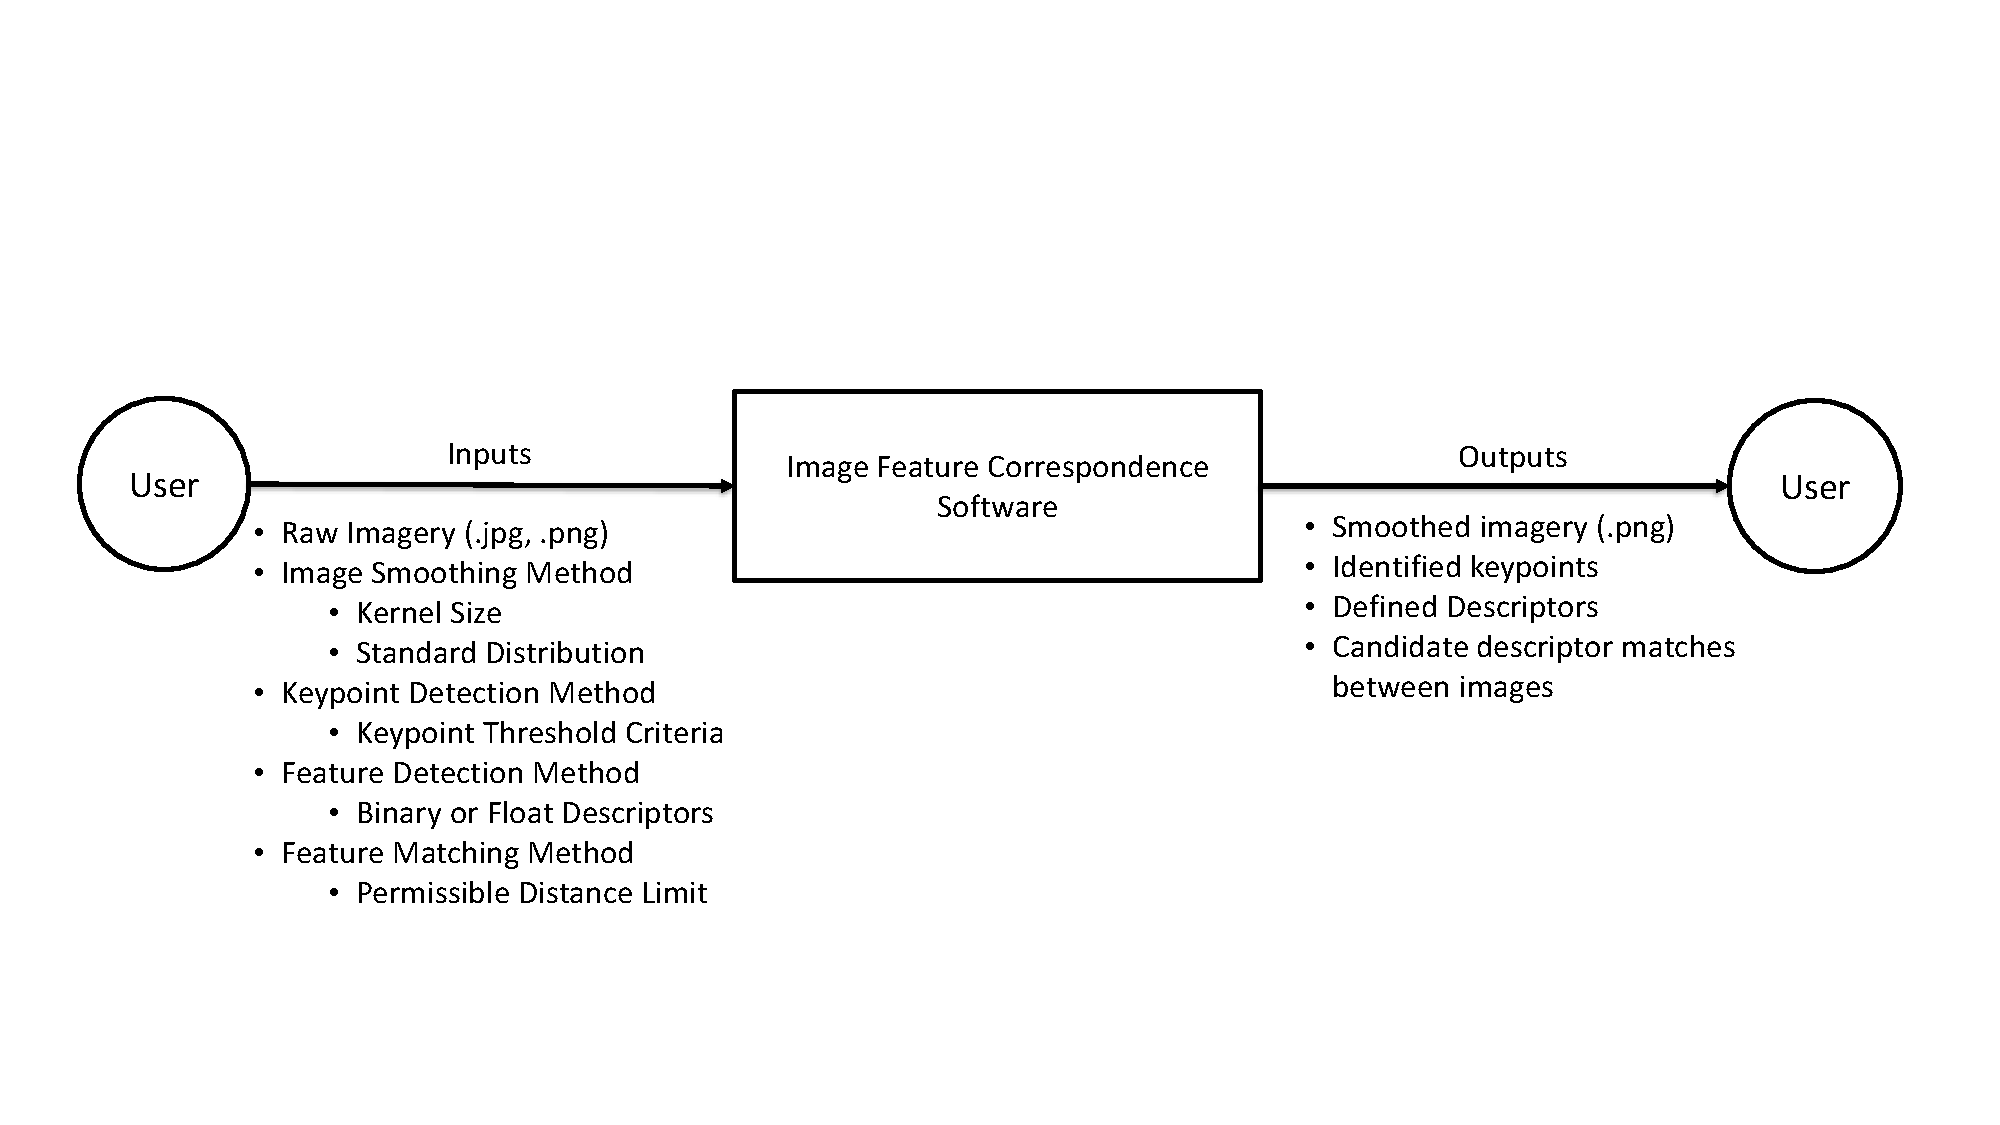
\includegraphics[width=1.0\textwidth]{SystemContextFigure}
\caption{System Context}
\label{Fig_SystemContext} 
\end{center}
\end{figure}

\begin{itemize}
\item User Responsibilities:
\item % Updated bullets to reflect the input as camera data
\begin{itemize}
\item Provide camera images to the system
\item Specific the desired methods of image smoothing, keypoint identification, definition of features from keypoints, and comparison of features
\item Refine the tuning parameters used for each of the specified processes
\item Verify that the input data is contained in the correct data structures
\item Configure the type of feature-handler algorithms to be used with corresponding 
threshold criteria
\end{itemize}
\item \progname{} Responsibilities:
\begin{itemize}
\item Detect data type mismatch, such as a string of characters instead of a floating point number
\item Assess whether inputs constitute a fully defined physical setup
\item Calculate match candidates between two images
\item Provide a quality metric of confidence in the calculated outputs
\end{itemize}
\end{itemize}
This software is not intended for use in safety-critical applications. If it is required for 
applications that are deemed to be safety-critical, then the software will need to undergo a new 
review and verification cycle.

\subsection{User Characteristics} \label{SecUserCharacteristics}
% updated per feedback on SRS Rev 1.0
As the intent of this software is intended to be used primarily in a research environment, 
the intended user is expected to posses a similar prerequisite knowledge base as that of the 
intended reader of the SRS, as outlined in Section \ref{sec_IntendedReader}. Therefore, the 
user of the IFC software should be familiar with the following prerequisite material outlined 
in Table \ref{Table_UserChar} prior to use of the software. 

\subsection{System Constraints}
The IFC software shall be compatible with Python 3.1 libraries, such as
OpenCV.

\section{Specific System Description}
This section first presents the problem description, which gives a high-level
view of the problem to be solved.  This is followed by the solution characteristics
specification, which presents the assumptions, theories, definitions and finally
the instance models. 

\subsection{Problem Description} \label{Sec_pd}

\progname{} is intended to evaluate how imagery data from robot-based cameras can 
can be manipulated to define and align features between separate images in support 
of downstream operations for extrinsic camera calibration.

\subsubsection{Terminology and  Definitions}

This subsection provides a list of terms that are used in the subsequent
sections and their meaning, with the purpose of reducing ambiguity and making it
easier to correctly understand the requirements:

\begin{itemize}

\item \textbf{Features:} distinctive patterns or structures in an image that are 
identifiable and useful for matching between images

\item \textbf{Keypoints:} specific pixel locations in an image that represent 
significant and repeatable features
\item \textbf{Correspondences:} pairs of keypoints between two images that represent 
represent the same real-world point
% typo updated
\item \textbf{Extrinsic Parameters:} the transform between the 3D camera frame to the 
3D world frame.
\item \textbf{Intrinsic Parameters:} camera parameters that pertain to the transform of the 
2D image plane frame to the 3D camera frame
\item \textbf{Hand-eye:} the relation between the robot end-effector to the camera frame
\item \textbf{Robot-world:} the relation between the robot base frame to the world frame
\item \textbf{Pose:} refers to the position and orientation of an object, sensor, or robot in $SE(3)$
\item \textbf{Patch:} a region of defined size ($p_{sz} \times p_{sz}$) that is used to compare pixels and define a feature descriptor
\end{itemize}


\subsubsection{Physical System Description} \label{sec_phySystDescrip}
% corrected pointers to figures
\noindent\label{PS_1}PS1: Frames for the robot base, hand, camera, and target landmark.\\
\noindent\label{PS_2}PS2: Known base-to-hand transform.\\
\noindent\label{PS_3}PS3: Projected camera images from distinct camera poses.\\ \\
The physical system of \progname{}, as shown in Figure \ref{Wang_EOH}, outlines 
case of a single-camera, single target configuration (PS1). This outlines the frames of 
interest for for the broader problem formulation. \\

\begin{figure}[h!]
  \begin{center}
  \centering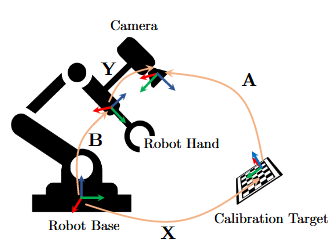
\includegraphics[width=0.45\textwidth]{Images/Wang_EOH.png}
  \caption{PS1: Single-camera robotic manipulator robot-world hand eye 
  configuration. Modified from \cite{Wang_2022}.}.
  \label{Wang_EOH}
  \end{center}
\end{figure}
\noindent The single-camera configuration can be extrapolated to the multi-camera, multi-target case (PS2), as shown in Figure \ref{OASIS}, from which a representation of equivalent keypoints between images (PS3) is shown in Figure \ref{MV_HZ}. The formulation in Figure \ref{MV_HZ} is what will be addressed by the IFC software.\\

\begin{figure}[h!]
  \begin{center}
  \centering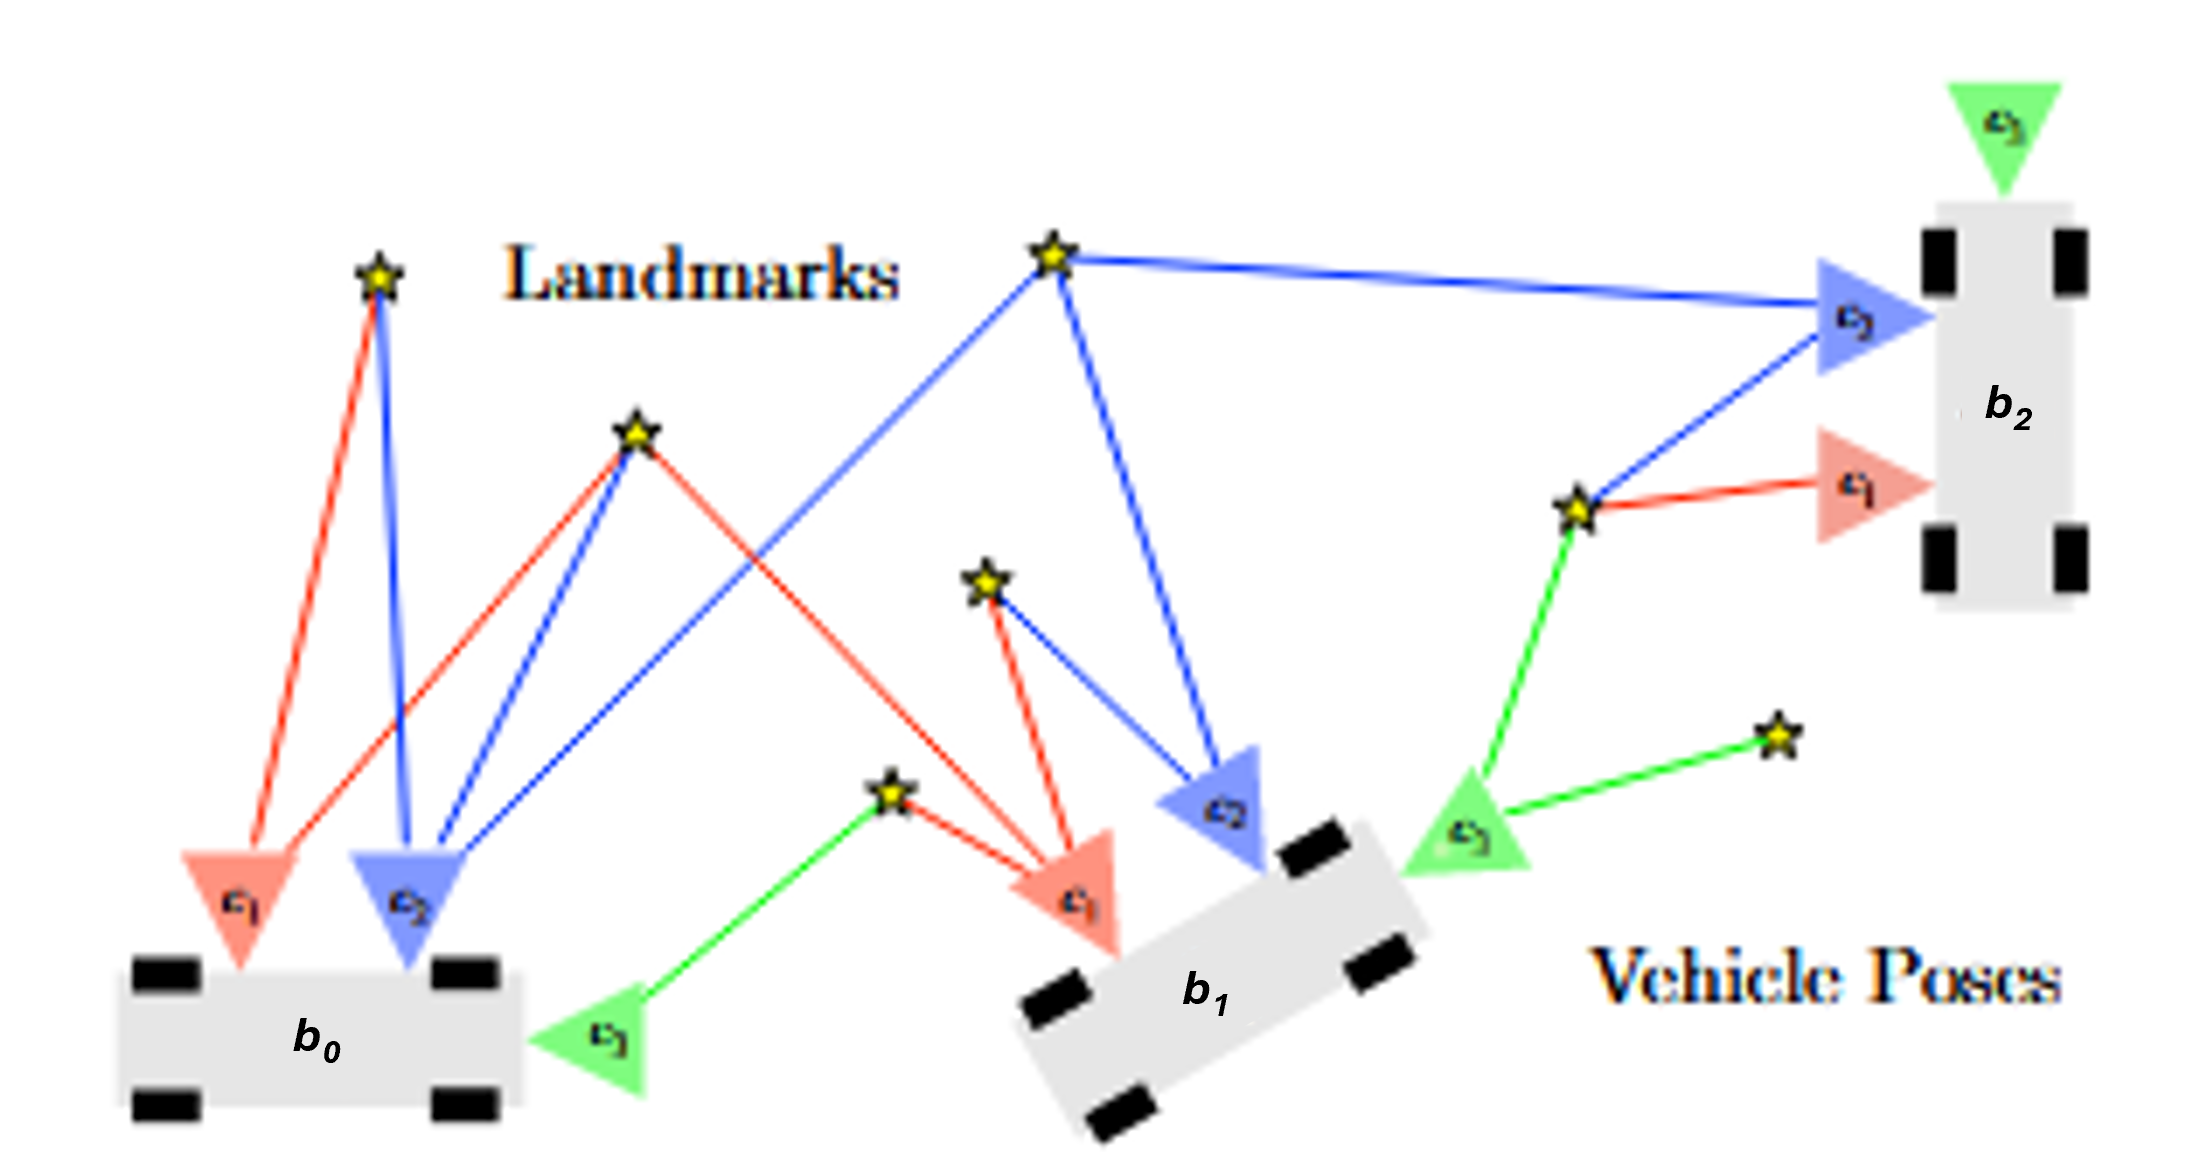
\includegraphics[width=0.45\textwidth]{Images/OASIS_RevVar.png}
  \caption{PS2: Multi-camera mobile robotic platform. 
  Modified from \cite{OASIS_2024}.}
  \label{OASIS}
  \end{center}
\end{figure}


\begin{figure}[h!]
  \begin{center}
  \centering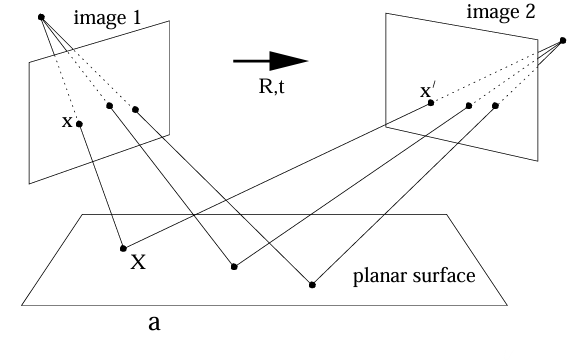
\includegraphics[width=0.45\textwidth]{Images/MULTIVIEW.png}
  \caption{PS3: Multi-camera mobile robotic platform. 
  Modified from \cite{Hartley_Zisserman}.}
  \label{MV_HZ}
  \end{center}
\end{figure}


\newpage
\subsubsection{Goal Statements}
\noindent The system goals follow.

\begin{itemize}
  % removed GS1 and GS2 from Rev 1.0
  \item[GS\refstepcounter{goalnum}\thegoalnum \label{identify_features}:]
    Identify a collection of features from each input image frame. 
  \item[GS\refstepcounter{goalnum}\thegoalnum \label{identify_matches}:] 
  % updated to specify the images for which features as assessed
    Identify feature correspondences between all input images.
  \item[GS\refstepcounter{goalnum}\thegoalnum \label{report_matches}:]
    Generate a report of the identified feature correspondences.
    
\end{itemize}

\subsection{Solution Characteristics Specification}
\begin{figure}[H]
  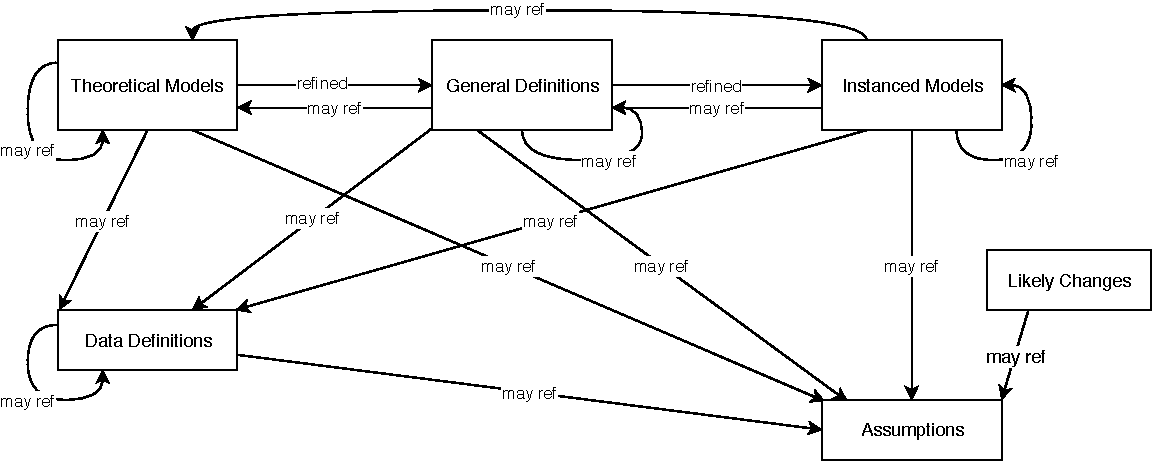
\includegraphics[scale=0.85]{RelationsBetweenTM_GD_IM_DD_A.pdf}
\end{figure}

The instance models that govern \progname{} are presented in
Section~\ref{sec_instance}.  The information to understand the meaning of the
instance models and their derivation is also presented, so that the instance
models can be verified.

\subsubsection{Types}
Omitted for Rev 1.0 release.

\subsubsection{Scope Decisions}
Control of the ambient illumination conditions falls outside the scope of this software.
It is the responsibility of the user to verify that the ambient lighting conditions do 
not change to a significant degree during the image capture process.


\subsubsection{Modelling Decisions}
Omitted for Rev 1.0 release.

\subsubsection{Assumptions} \label{sec_assumpt}
This section simplifies the original problem and helps in developing the
theoretical model by filling in the missing information for the physical system.
The numbers given in the square brackets refer to the theoretical model [TM],
general definition [GD], data definition [DD], instance model [IM], or likely
change [LC], in which the respective assumption is used.

\begin{itemize}
\item[A\refstepcounter{assumpnum}\theassumpnum \label{A_min_num_cameras}:]
Imagery shall be provided by at least one camera (\dref{TM_Dist_Ham}).

\item[A\refstepcounter{assumpnum}\theassumpnum \label{A_camera_model}:]
All supplied imagery is produced by a pinhole model, affine camera 
(\tref{TM_FAST}, , \dref{GD_2D_Gauss}).

\item[A\refstepcounter{assumpnum}\theassumpnum \label{A_greyscale}:]
All imagery will be input as greyscale data (\dref{GD_2D_Gauss}).

\item[A\refstepcounter{assumpnum}\theassumpnum \label{A_RT_Memory}:]
The solution is not limited to memory constraints observed in hardware used for real-time 
applications (\tref{TM_BRIEF}).

\end{itemize}

\subsubsection{Theoretical Models}\label{sec_theoretical}
This section introduces the general equations and laws that are used to build the 
\progname{} software.

~\newline



% Theoretical Model 1
\noindent
\begin{minipage}{\textwidth}
\renewcommand*{\arraystretch}{1.5}
\begin{tabular}{| p{\colAwidth} | p{\colBwidth}|}
\hline
\rowcolor[gray]{0.9}
Number & TM\refstepcounter{theorynum}\thetheorynum \label{TM_ND_Gauss} \\
\hline
Label & \textbf{N-Dimensional Gaussian Kernel} \\
\hline
Equation & $G_{\text{N-Dim}}(x,\sigma) = \frac{1}{2\pi\sigma^2} \exp\left(-\frac{\|\vec{x}\|^2}{2\sigma^2}\right)$ \\
\hline
Description & 
$G_{\text{N-Dim}}$ represents the probability density function of an $n$-dimensional Gaussian distribution. 
$\vec{x}$ is the $n$-dimensional input vector, and $\sigma$ is the standard deviation controlling the spread of the distribution. 
This kernel is often used in smoothing, weighting, and noise modeling. \\
\hline
Notes & All variables are unitless. \\
\hline
Source & \cite{Gauss_Kernel} \\
\hline
Ref.\ By & \dref{GD_2D_Gauss} \\
\hline
Pre-conditions for TM\thetheorynum: & None \\
\hline
Derivation for TM\thetheorynum: & None \\
\hline
\end{tabular}
\end{minipage}\\


% Theoretical Model 2
\noindent
\begin{minipage}{\textwidth}
\renewcommand*{\arraystretch}{1.5}
\begin{tabular}{| p{\colAwidth} | p{\colBwidth}|}
\hline
\rowcolor[gray]{0.9}
Number & TM\refstepcounter{theorynum}\thetheorynum \label{TM_FAST} \\
\hline
Label & \textbf{Features from Accelerated Segment Test (FAST)} \\
\hline
Equation & $S = \sum_{i \in x} \left( |I(p) - I(x_i)| > t \right) > 12$ \\
\hline
Description & 
For a 2D image acquired via a pinhole affine camera model (\aref{A_camera_model}), $p$ denotes the central pixel of interest, and $x = \{x_1, \dots, x_{16}\}$ are the 16 contiguous pixels forming a circle around $p$. \\
& $I(p)$ and $I(x_i)$ are the pixel intensities at locations $p$ and $x_i$, respectively. \\
& $t$ is a user-defined intensity threshold. The segment test $S$ counts how many surrounding pixels differ from $p$ by more than $t$. If more than 12 such pixels are found, $p$ is identified as a keypoint. \\
\hline
Notes & All variables are unitless. \\
\hline
Source & \cite{FAST} \\
\hline
Ref.\ By & \dref{GD_FAST}, \lcref{LC_keypoint_method} \\
\hline
Pre-conditions for TM\thetheorynum: & None \\
\hline
Derivation for TM\thetheorynum: & None \\
\hline
\end{tabular}
\end{minipage}\\



% Theoretical Model 3
\noindent
\begin{minipage}{\textwidth}
\renewcommand*{\arraystretch}{1.5}
\begin{tabular}{| p{\colAwidth} | p{\colBwidth}|}
\hline
\rowcolor[gray]{0.9}
Number & TM\refstepcounter{theorynum}\thetheorynum \label{TM_BRIEF} \\
\hline
Label & \textbf{Binary Robust Independent Elementary Features (BRIEF)} \\
\hline
Equation & 
$\mathbf{d} = \{d_1, d_2, \dots, d_{256}\}, \quad 
\text{where } d_k = 
\begin{cases}
1 & \text{if } I(p_{k1}) < I(p_{k2}) \\
0 & \text{otherwise}
\end{cases}$ \\
\hline
Description & 
$\mathbf{d}$ is a 256-bit (32-byte) binary descriptor vector. 
To compute each bit $d_k$, a square patch of size $p_{sz} \times p_{sz}$ is centered at a detected keypoint. 
Two pixels, $p_{k1}$ and $p_{k2}$, are randomly sampled from this patch. 
If the intensity at $p_{k1}$ is less than that at $p_{k2}$, $d_k$ is set to 1; otherwise, it is set to 0. \\
\hline
Notes & BRIEF is efficient but may not be suitable for real-time applications under strict memory constraints (\aref{A_RT_Memory}). \\
\hline
Source & \cite{opencv_orb_tutorial} \\
\hline
Ref.\ By & \dref{GD_rBRIEF}, \lcref{LC_descriptor_method} \\
\hline
Pre-conditions for TM\thetheorynum: & None \\
\hline
Derivation for TM\thetheorynum: & None \\
\hline
\end{tabular}
\end{minipage}\\




~\newline

% Theoretical Model 4
\noindent
\begin{minipage}{\textwidth}
\renewcommand*{\arraystretch}{1.5}
\begin{tabular}{| p{\colAwidth} | p{\colBwidth}|}
\hline
\rowcolor[gray]{0.9}
Number & TM\refstepcounter{theorynum}\thetheorynum \label{TM_Dist_Ham} \\
\hline
Label & \textbf{Hamming Distance} \\
\hline
Equation & 
$d_{\text{Hamming}}(\mathbf{d}_{\alpha}, \mathbf{d}_{\beta}) = \sum_{i=0}^{n-1} \left( d_{\alpha, i} \oplus d_{\beta, i} \right)$ \\
\hline
Description & 
The Hamming distance measures the number of differing bits between two binary descriptors, $\mathbf{d}_{\alpha}$ and $\mathbf{d}_{\beta}$. \\
& Each descriptor is composed of $n$ bits. The bitwise exclusive-OR operation ($\oplus$) is used to compare corresponding bits. \\
& The total number of differing bits is returned as an integer. This is not a geometric distance, but a metric in Hamming space. \\
\hline
Notes & All variables are unitless. \\
\hline
Source & \cite{opencv_flann_matcher} \\
\hline
Ref.\ By & \iref{IM_Dist_Hamm}, \lcref{LC_comparison_method} \\
\hline
Pre-conditions for TM\thetheorynum: & None \\
\hline
Derivation for TM\thetheorynum: & None \\
\hline
\end{tabular}
\end{minipage}\\


~\newline

\subsubsection{General Definitions}\label{sec_gendef}
This section collects the laws and equations that will be used in building the
instance models.

~\newline

% General Definition 1
% updated per comment to clarify derivation
\noindent
\begin{minipage}{\textwidth}
\renewcommand*{\arraystretch}{1.5}
\begin{tabular}{| p{\colAwidth} | p{\colBwidth}|}
\hline
\rowcolor[gray]{0.9}
Number & GD\refstepcounter{defnum}\thedefnum \label{GD_2D_Gauss} \\
\hline
Label & \textbf{2-Dimensional Gaussian Kernel} \\
\hline
SI Units & Unitless \\
\hline
Equation & 
$G_{2D}(u, v, \sigma) = \frac{1}{2\pi\sigma^2} \exp\left(-\frac{u^2 + v^2}{2\sigma^2}\right)$ \\
\hline
Description & 
$G_{2D}$ represents the 2D Gaussian kernel function applied to a grayscale image 
(\aref{A_camera_model}, \aref{A_greyscale}). 
The variables $u$ and $v$ denote the horizontal and vertical distances from the kernel center, respectively (both are unitless). 
The parameter $\sigma$ represents the standard deviation of the Gaussian distribution, which controls the amount of smoothing applied. 
This kernel is convolved with the image to reduce high-frequency noise and enhance regional uniformity. \\
\hline
Source & TM\ref{TM_ND_Gauss} \\
\hline
Ref.\ By & \iref{IM_GK} \\
\hline
\end{tabular}
\end{minipage}\\


~\newline

% General Defintion 2
\noindent
\begin{minipage}{\textwidth}
\renewcommand*{\arraystretch}{1.5}
\begin{tabular}{| p{\colAwidth} | p{\colBwidth}|}
\hline
\rowcolor[gray]{0.9}
Number& GD\refstepcounter{defnum}\thedefnum \label{GD_FAST}\\
\hline
Label &\bf FAST Implementation \\
\hline
Units&Unitless\\
\hline
Equation&$\mathit{\sum\limits_{k \in x} (|I_{k} - I(u,v)|>t) \geq N}$  \\
\hline
Description &  The threshold count of $\mathit{x \in \{1 \dots 16 \}}$ is concretely defined as $\mathit{N}$. 
$\mathit{I(u,v)}$ represents the pixel intensity of pixel $\mathit{p}$. $\mathit{I_{k}}$ represents 
the grayscale image intensity of the $k^{th}$ pixel in the circle around pixel $\mathit{p}$. 
$\mathit{t}$ represents the user-defined threshold to define an allowable range of pixel intensity.
\\
\hline
  Source & TM\ref{TM_FAST} \\
  \hline
  Ref.\ By & \iref{IM_GK}\\
  \hline
\end{tabular}
\end{minipage}\\



% General Definition 3
\noindent
\begin{minipage}{\textwidth}
\renewcommand*{\arraystretch}{1.5}
\begin{tabular}{| p{\colAwidth} | p{\colBwidth} |}
\hline
\rowcolor[gray]{0.9}
Number & GD\refstepcounter{defnum}\thedefnum \label{GD_rBRIEF} \\
\hline
Label & \textbf{Rotated BRIEF} \\
\hline
Units & Unitless \\
\hline
Equation & 
$d_k = 
\begin{cases}
1 & \text{if } I(p_{k1}') < I(p_{k2}') \\
0 & \text{otherwise}
\end{cases}$ \\
\hline
Description & 
$\mathit{d_k}$ represents the $k^{th}$ bit in the BRIEF descriptor. 
For each bit, two points $p_{k1}'$ and $p_{k2}'$ are selected within a patch centered at the keypoint. 
These point pairs are generated by rotating a canonical sampling pattern according to the keypoint's orientation. 
This process ensures that BRIEF descriptors are invariant to in-plane rotations. \\
\hline
Source & \cite{opencv_orb_tutorial} \\
\hline
Ref.\ By & \iref{IM_BRIEF_Desc} \\
\hline
\end{tabular}
\end{minipage}\\




\subsubsection*{Detailed derivation of Rotated Brief Transform}
$\mathit{p_{k}}$ and $\mathit{q_{k}}$ are calculated by successive increments of a 12\textdegree. 
The transform between $\mathit{p_{k}^{'}}$ and $\mathit{q_{k}^{'}}$ is outlined below, where $\theta$ 
represents the increase in rotation by a denomination of 12\textdegree. \\

\[
\begin{bmatrix} p_k' \\ q_k' \end{bmatrix} =
\begin{bmatrix} \cos\theta & -\sin\theta \\ \sin\theta & \cos\theta \end{bmatrix}
\begin{bmatrix} p_k \\ q_k \end{bmatrix}
\]

\subsubsection{Data Definitions}\label{sec_datadef}
No data definitions are outlined for the current release.

\subsubsection{Instance Models} \label{sec_instance}    
This section transforms the problem defined in Section~\ref{Sec_pd} into 
one which is expressed in mathematical terms. It uses refined derivations of the 
models outlined in Sections~\ref{sec_theoretical} and~\ref{sec_gendef}.

~\newline

%Instance Model 1
\noindent
\begin{minipage}{\textwidth}
\renewcommand*{\arraystretch}{1.5}
\begin{tabular}{| p{\colAwidth} | p{\colBwidth}|}
  \hline
  \rowcolor[gray]{0.9}
  Number & IM\refstepcounter{instnum}\theinstnum \label{IM_GK} \\
  \hline
  Label & \textbf{Gaussian-Smoothed Image, $\mathcal{I'}_{i,j}(u,v,\sigma)$} \\
  \hline
  Input & $\mathcal{I}_{i,j}(u,v)$, the raw grayscale image from \tref{TM_ND_Gauss} \\ 
        & $G_{2D}(x,y,\sigma)$, the 2D Gaussian kernel from \dref{GD_2D_Gauss} \\
  \hline
  Output & $\mathcal{I'}_{i,j}(u,v,\sigma)$, the Gaussian-smoothed image \\
  \hline
  Equation & 
  $\mathcal{I'}_{i,j}(u,v,\sigma) = \sum_{x=-k}^{k} \sum_{y=-k}^{k} G_{2D}(x,y,\sigma) \cdot \mathcal{I}_{i,j}(u-x, v-y)$ \\[1ex]
  \hline
  Description & 
  $\mathcal{I'}_{i,j}(u,v,\sigma)$ is the output image obtained by convolving the input image $\mathcal{I}_{i,j}(u,v)$ with a Gaussian kernel $G_{2D}(x,y,\sigma)$ of size $(2k+1)\times(2k+1)$. \\
  & 
  The kernel size is selected based on the standard deviation $\sigma$, and defines the smoothing window centered at pixel $(u,v)$. \\
  & 
  The convolution suppresses high-frequency components (e.g., noise), producing a smoother version of the input image. \\
  \hline
  Sources & \cite{Gauss_Kernel} \\
  \hline
  Ref.\ By & \gsref{identify_features}, \gsref{identify_matches}, \iref{IM_FAST_Detect} \\
  \hline
\end{tabular}
\end{minipage}\\


~\newline

% Instance Model 2
\noindent
\begin{minipage}{\textwidth}
\renewcommand*{\arraystretch}{1.5}
\begin{tabular}{| p{\colAwidth} | p{\colBwidth}|}
  \hline
  \rowcolor[gray]{0.9}
  Number & IM\refstepcounter{instnum}\theinstnum \label{IM_FAST_Detect} \\
  \hline
  Label & \textbf{Image Keypoint Detection, $\mathcal{D}_{i,j}(u,v)$} \\
  \hline
  Input & $\mathcal{I}_{i,j}(u,v,\sigma)$ from \iref{IM_GK}, intensity threshold $t$ \\
  \hline
  Output & $\mathcal{D}_{i,j}(u,v)$ — a set of keypoints, each defined by pixel coordinates $(u,v)$ in the image plane. \\
  \hline
  Description & 
  $\mathcal{D}_{i,j}(u,v)$ represents the set of image keypoints detected in the smoothed grayscale image 
  $\mathcal{I}_{i,j}(u,v,\sigma)$ using the FAST algorithm described in \tref{TM_FAST}. \\
  & Each keypoint corresponds to a pixel location $(u,v)$ for which the segment test $S$ exceeds a count of 12, 
  indicating a corner-like intensity pattern around that pixel. \\
  & $t$ is the user-defined pixel intensity threshold that determines contrast sensitivity. \\
  \hline
  Sources & \cite{FAST} \\
  \hline
  Ref.\ By & \gsref{identify_features}, \iref{IM_BRIEF_Desc} \\
  \hline
\end{tabular}
\end{minipage}\\


~\newline

% Instance Model 3
\noindent
\begin{minipage}{\textwidth}
\renewcommand*{\arraystretch}{1.5}
\begin{tabular}{| p{\colAwidth} | p{\colBwidth}|}
  \hline
  \rowcolor[gray]{0.9}
  Number & IM\refstepcounter{instnum}\theinstnum \label{IM_BRIEF_Desc} \\
  \hline
  Label & \textbf{Produce Feature Descriptors, $\mathit{D_{bin}}$} \\
  \hline
  Input & $\mathcal{D}_{i,j}(u,v)$ from \iref{IM_FAST_Detect}, $p_{sz}$, $l_{bin}$ \\
  \hline
  Output & $\mathit{D_{bin}}$, a variable-length vector of binary feature descriptors \\
  \hline
  Description & 
  $\mathcal{D}_{i,j}(u,v)$ is the set of keypoints defined by their pixel coordinates, as obtained from \iref{IM_FAST_Detect}. \\
  & $p_{sz}$ is the size of the square pixel patch (in pixels) used to compute each descriptor. \\
  & $l_{bin}$ specifies the number of binary comparisons (i.e., bits) to generate per descriptor, as required by \tref{TM_BRIEF}. \\
  & $\mathit{D_{bin}}$ is the resulting collection of BRIEF descriptors, each computed from randomly sampled pixel pairs within a patch centered on a keypoint. \\
  \hline
  Sources & \cite{opencv_orb_tutorial} \\
  \hline
  Ref.\ By & \gsref{identify_matches}, \iref{IM_Dist_Hamm} \\
  \hline
\end{tabular}
\end{minipage}\\


~\newline

% Instance Model 4
\noindent
\begin{minipage}{\textwidth}
\renewcommand*{\arraystretch}{1.5}
\begin{tabular}{| p{\colAwidth} | p{\colBwidth}|}
  \hline
  \rowcolor[gray]{0.9}
  Number & IM\refstepcounter{instnum}\theinstnum \label{IM_Dist_Hamm} \\
  \hline
  Label & \textbf{Inter-Image Descriptor Comparison, $\mathit{dist_{Hamming}}$} \\
  \hline
  Input & $\mathit{d_a}$, $\mathit{d_b}$ from \iref{IM_BRIEF_Desc} \\
  \hline
  Output & $\mathit{dist_{Hamming}}$, an integer value \\
  \hline
  Description & 
  $\mathit{d_a}$ and $\mathit{d_b}$ are binary descriptors generated from different keypoints, as defined in \iref{IM_BRIEF_Desc}. \\
  & $\mathit{dist_{Hamming}}$ is computed as the Hamming distance between these descriptors, equal to the number of differing bits. \\
  & Each bit-wise comparison uses the exclusive-OR operator ($\oplus$), as formalized in \tref{TM_Dist_Ham}. \\
  \hline
  Sources & \cite{opencv_flann_matcher} \\
  \hline
  Ref.\ By & \gsref{identify_matches} \\
  \hline
\end{tabular}
\end{minipage}\\




\subsubsection{Input Data Constraints} \label{sec_DataConstraints}    

Table~\ref{TblInputVar} shows the data constraints on the input output
variables.  The column for physical constraints gives the physical limitations
on the range of values that can be taken by the variable.  The column for
software constraints restricts the range of inputs to reasonable values.  The
software constraints will be helpful in the design stage for picking suitable
algorithms.  The constraints are conservative, to give the user of the model the
flexibility to experiment with unusual situations.  The column of typical values
is intended to provide a feel for a common scenario.  The uncertainty column
provides an estimate of the confidence with which the physical quantities can be
measured.  This information would be part of the input if one were performing an
uncertainty quantification exercise.

The specification parameters are outlined in Table~\ref{TblInputVar}.

\begin{table}[!h]
  \caption{Input Variables} \label{TblInputVar}
  \renewcommand{\arraystretch}{1.2}
\noindent \begin{longtable*}{l l l l c} 
  \toprule
  \textbf{Var} & \textbf{Physical Constraints} & \textbf{Software Constraints} &
                             \textbf{Typical Value} & \textbf{Uncertainty}\\
  \midrule 
  $\mathit{\mathcal{I}_{i, j}(u,v)}$ & N/A & $0 \leq \mathit{\mathcal{I}_{i, j}(u,v)} \leq 255$ 
  & N/A & N/A  % at least one camera
  \\
  $\sigma$ & $\sigma > 0$ & $\sigma > 0 $ & 0.05 & N/A % std dev > 0
  \\
  \bottomrule
\end{longtable*}
\end{table}
\noindent 
\begin{description}
\item[(*)] $\mathit{\mathcal{I}_{i, j}(u,v)}$ is limited to being an 8-bit unsigned integer
\item[(*)] standard deviation, $\sigma$, is constrained to be positive and real
% eliminated robot pose limits
\end{description}

\subsubsection{Properties of a Correct Solution} \label{sec_CorrectSolution}

\noindent
Each image needs to be assessed such that it is invariant to the order for which it is processed by the software. In other words, the output of the \progname{} software should be deterministic. Each identified keypoint needs to have an associated set of pixel coordinates. Each descriptor needs to have an associated keypoint and unique identifier. Each candidate match between features needs to have associated keypoints, descriptors, and identifiers for the points of origin of both consituitive images.

\noindent
\\
\\
As it stands, there are currently no 
identified physical constraints on the system.


\section{Requirements}\label{Header_Req}
This section provides the functional requirements, the business tasks that the
software is expected to complete, and the nonfunctional requirements, the
qualities that the software is expected to exhibit.

\subsection{Functional Requirements}

\noindent \begin{itemize}

% Inputs
\item[R\refstepcounter{reqnum}\thereqnum \label{R_Update_SD}:] The IFC software shall accept 
updates to the variance in image noise,  $\mathit{\sigma}$, upon user input.

\item[R\refstepcounter{reqnum}\thereqnum \label{R_Update_Intensity}:] The IFC software shall accept 
updates to the image intensity threshold, $\mathit{t}$, upon user input.

\item[R\refstepcounter{reqnum}\thereqnum \label{R_Update_Patch}:] The IFC software shall accept 
updates to the patch size, $\mathit{p_{s}}$, upon user input.

\item[R\refstepcounter{reqnum}\thereqnum \label{R_Update_BinSize}:] The IFC software shall accept 
updates to the bin size, $\mathit{l_{bin}}$, upon user input.

\item[R\refstepcounter{reqnum}\thereqnum \label{R_Default_Noise}:] The IFC software shall use a 
default noise suppresion parameter of $\sigma = 1$ if no option is specified by the user.

\item[R\refstepcounter{reqnum}\thereqnum \label{R_Default_FD}:] The IFC software shall use corner 
detection as the default feature detection method if no option is specified by the user.

\item[R\refstepcounter{reqnum}\thereqnum \label{R_Default_KD}:] The IFC software shall use binary 
descriptors as the default keypoint descriptor method if no option is specified by the user.

\item[R\refstepcounter{reqnum}\thereqnum \label{R_Default_FM}:] The IFC software shall use compare 
feature descriptors by their Hamming Distance if no alternative descriptor matching method 
is specified by the user.

% Calculations 
\item[R\refstepcounter{reqnum}\thereqnum \label{R_NoiseReduction}:] The IFC software shall 
implement noise reduction on an input greyscale image per a prescribed standard deviation (from 
\iref{IM_GK}).

\item[R\refstepcounter{reqnum}\thereqnum \label{R_DetectKeypoints}:] The IFC software shall, given a 2D 
greyscale image, define a set of keypoints per the alloted threshold criteria (from 
\iref{IM_FAST_Detect}).

\item[R\refstepcounter{reqnum}\thereqnum \label{R_DefineDescriptors}:] The IFC software shall 
define feature descriptors from identified keypoints (from \iref{IM_BRIEF_Desc}).

\item[R\refstepcounter{reqnum}\thereqnum \label{R_CompareDescriptors}:] The IFC software shall 
identify matches between descriptors that originate from separate images (from \iref{IM_Dist_Hamm}).

\item[R\refstepcounter{reqnum}\thereqnum \label{R_DistinctImages}:] The IFC software shall review 
all identified feature matches to confirm that they originate from separate images.

% Outputs 
% Verify Outputs
\item[R\refstepcounter{reqnum}\thereqnum \label{R_UniqueMatch_IDs}:] The IFC software shall report 
that all feature correspondences are uniquely defined by two respective sets of cameras and pose 
frames as an output.

\item[R\refstepcounter{reqnum}\thereqnum \label{R_OutputCorrespondences}:] The IFC software shall report 
the identified matches between features, with corresponding camera and pose identifiers, as an output.

\end{itemize}

\subsection{Nonfunctional Requirements}

\noindent \begin{itemize}

\item[NFR\refstepcounter{nfrnum}\thenfrnum \label{NFR_Rel_1}:] \textbf{Reliability}
The IFC software shall be invariant to the order that imagery data is provided to the feature 
matching process.

\item[NFR\refstepcounter{nfrnum}\thenfrnum \label{NFR_Use_1}:] \textbf{Usability}
The IFC system shall provide an interface that at least 80\% of its users would describe 
as 'simple to use' based on direct feedback.

\item[NFR\refstepcounter{nfrnum}\thenfrnum \label{NFR_Mtn_1}:] \textbf{Maintainability}
The IFC software should support implementation of new feature detection methods within 30\% 
of the total time effort required to develop the default method of feature detection.

\item[NFR\refstepcounter{nfrnum}\thenfrnum \label{NFR_Perf_1}:] \textbf{Performance}
The IFC software should report timing metrics for each image processing operation.

\item[NFR\refstepcounter{nfrnum}\thenfrnum \label{NFR_Perf_2}:] \textbf{Performance}
The system should report the average and maximum memory used during each operation.


\end{itemize}

\subsection{Rationale}

The scope and assumptions of this document are intended to encapsulate a realistic problem formulation 
software. This software is intended for use in laboratory experimentation and configurations, rather than 
as an off-the-shelf product for applications that involve more risk, such as those that are safety-critical 
or mission critical in scope.\\ \\
A\ref{A_min_num_cameras} is necessary at it enables flexibility to developers to scale the software to the case of multiple cameras in the event that the use case of a single camera can be successfully implemented. However, it does not specify that support for multiple cameras is necessary. A\ref{A_camera_model} is necessary as all imagery needs to be projected on a 2D affine plane as the software is not intended to be used with imagery that is procurred using a fish-eye lens. A\ref{A_greyscale} is necessary as it significant reduces the complexity of computation that is required to process colour imagery. Conversion to greyscale is a standard industrial practice for image processing. A\ref{A_RT_Memory} is necessary to avoid imposing timing and performance constraints on the software. This would consitute the need to perform a hazard analysis to address safety and performance challenges that would arise from operating in a real-time scenario. 

\section{Likely Changes} 
\noindent \begin{itemize}

\item[LC\refstepcounter{lcnum}\thelcnum\label{LC_keypoint_method}:] 
The theoretical model of keypoint detection will be abstracted to expand the types of 
implementation models that can be used.

\item[LC\refstepcounter{lcnum}\thelcnum\label{LC_descriptor_method}:] 
The theoretical model of assigning feature descriptors will be abstracted to expand the types of 
implementation models that can be used.

\item[LC\refstepcounter{lcnum}\thelcnum\label{LC_comparison_method}:] 
The theoretical model of descriptor matching will be abstracted to expand the types of 
implementation models that can be used.

\end{itemize}

\section{Unlikely Changes}    

\noindent \begin{itemize}

\item[LC\refstepcounter{lcnum}\thelcnum\label{RGB_Data}:] It is unlikely that the design 
will need to be adjusted to perform computation on RGB data instead of grayscale data.

\end{itemize}

\section{Traceability Matrices and Graphs}

The purpose of the traceability matrices is to provide easy references on what
has to be additionally modified if a certain component is changed.  Every time a
component is changed, the items in the column of that component that are marked
with an ``X'' may have to be modified as well.  Table~\ref{Table:trace} shows the
dependencies of theoretical models, general definitions, data definitions, and
instance models with each other. Table~\ref{Table:R_trace} shows the
dependencies of instance models, requirements, and data constraints on each
other. Table~\ref{Table:A_trace} shows the dependencies of theoretical models,
general definitions, data definitions, instance models, and likely changes on
the assumptions.

\afterpage{
\begin{landscape}
\begin{table}[h!]
\centering
\begin{tabular}{|c|c|c|c|c|c|c|c|c|c|c|c|c|c|c|c|c|c|c|c|}
\hline
	& \aref{A_min_num_cameras}& \aref{A_camera_model}& \aref{A_greyscale}& \aref{A_RT_Memory}\\
\hline
\tref{TM_ND_Gauss}              & & &X& \\ \hline
\tref{TM_FAST}                  & &X& & \\ \hline
\tref{TM_BRIEF}                 & &X& &X\\ \hline
\tref{TM_Dist_Ham}              &X& & & \\ \hline 
\dref{GD_2D_Gauss}              & &X& & \\ \hline
\dref{GD_FAST}                  & & & & \\ \hline
\dref{GD_rBRIEF}                & & & & \\ \hline
\iref{IM_GK}                    & & & & \\ \hline
\iref{IM_FAST_Detect}           & & & & \\ \hline
\iref{IM_BRIEF_Desc}            & & & & \\ \hline
\iref{IM_Dist_Hamm}             & & & & \\ \hline
\lcref{LC_keypoint_method}      & & & & \\ \hline
\lcref{LC_descriptor_method}    & & & & \\ \hline
\lcref{LC_comparison_method}    & & & & \\ \hline
\hline
\end{tabular}
\caption{Traceability Matrix Showing the Connections Between Assumptions and Other Items}
\label{Table:A_trace}
\end{table}
\end{landscape}
}

\begin{landscape}
\begin{table}[h!]
\centering
\begin{tabular}{|c|c|c|c|c|c|c|c|c|c|c|c|c|c|c|}
\hline        
& \tref{TM_ND_Gauss}& \tref{TM_FAST}& \tref{TM_BRIEF}& \tref{TM_Dist_Ham}& 
\dref{GD_2D_Gauss} & \dref{GD_FAST}  & \dref{GD_rBRIEF} &
\iref{IM_GK} & \iref{IM_FAST_Detect}& \iref{IM_BRIEF_Desc}& \iref{IM_Dist_Hamm}&
\lcref{LC_keypoint_method} & \lcref{LC_descriptor_method} & \lcref{LC_comparison_method}\\
\hline
\tref{TM_ND_Gauss}              & & & & &X& & &X& & & & & & \\ \hline
\tref{TM_FAST}                  & & & & & &X& & &X& & &X& & \\ \hline
\tref{TM_BRIEF}                 & & & & & & &X& & &X& & &X& \\ \hline
\tref{TM_Dist_Ham}              & & & & & & & & & & &X& & &X\\ \hline
\dref{GD_2D_Gauss}              & & & & & & & &X& & & & & & \\ \hline
\dref{GD_FAST}                  & & & & & & & & &X& & & & & \\ \hline
\dref{GD_rBRIEF}                & & & & & & & & & &X& & & & \\ \hline
\iref{IM_GK}                    & & & & & & & & &X& & & & & \\ \hline
\iref{IM_FAST_Detect}           & & & & & & & & & &X& & & & \\ \hline
\iref{IM_BRIEF_Desc}            & & & & & & & & & & &X& & & \\ \hline
\iref{IM_Dist_Hamm}             & & & & & & & & & & & & & & \\ \hline
\lcref{LC_keypoint_method}      & & & & & &X& & &X& & & & & \\ \hline
\lcref{LC_descriptor_method}    & & & & & & &X& & &X& & & & \\ \hline
\lcref{LC_comparison_method}    & & & & & & & & & & &X& & & \\ \hline
\hline
\end{tabular}
\caption{Traceability Matrix Showing the Connections Between Items of Different Sections}
\label{Table:trace}
\end{table}
\end{landscape}




\begin{landscape}
\begin{table}[h!]
\centering
\begin{tabular}{|c|c|c|c|c|c|c|c|c|c|c|c|c|c|c|c|c|c|c|c|c|c|c|}
\hline
	& \iref{IM_GK} & \iref{IM_FAST_Detect}& \iref{IM_BRIEF_Desc}& \iref{IM_Dist_Hamm}
  & \rref{R_Update_SD} &\rref{R_Update_Intensity} &\rref{R_Update_Patch} &\rref{R_Update_BinSize}
  & \rref{R_Default_Noise} &\rref{R_Default_FD} & \rref{R_Default_KD} 
  & \rref{R_Default_FM} &\rref{R_NoiseReduction}  &\rref{R_DetectKeypoints} 
  & \rref{R_DefineDescriptors} &\rref{R_CompareDescriptors} &\rref{R_DistinctImages}
  & \rref{R_UniqueMatch_IDs} &\rref{R_OutputCorrespondences} \\
\hline
                              % I1I2I3I4 1 2 3 4 5 6 7 8 9 101112131415
\iref{IM_GK}                    & &X& & &X& & & &X& & & &X& & & & & & \\ \hline
\iref{IM_FAST_Detect}           & & &X& & &X& & & &X& & & &X& & & & & \\ \hline
\iref{IM_BRIEF_Desc}            & & & &X& & &X&X& & &X& & & &X& & & & \\ \hline
\iref{IM_Dist_Hamm}             & & & & & & & & & & & &X& & & &X&X&X&X\\ \hline
\rref{R_Update_SD}              &X& & & & & & & & & & & &X& & & & & & \\ \hline
\rref{R_Update_Intensity}       & &X& & & & & & & & & & & &X& & & & & \\ \hline
\rref{R_Update_Patch}           & & &X& & & & & & & & & & & &X& & & & \\ \hline
\rref{R_Update_BinSize}         & & &X& & & & & & & & & & & &X& & & & \\ \hline
\rref{R_Default_Noise}          & & & & & & & & & & & & &X& & & & & & \\ \hline
\rref{R_Default_FD}             &X& & & & & & & & & & & & &X& & & & & \\ \hline
\rref{R_Default_KD}             & &X& & & & & & & & & & & & &X& & & & \\ \hline
\rref{R_Default_FM}             & & &X& & & & & & & & & & & & &X& & & \\ \hline
\rref{R_NoiseReduction}         &X& & & & & & & & & & & &X& & & & & & \\ \hline
\rref{R_DetectKeypoints}        & &X& & & & & & & & & & & & & & & & & \\ \hline
\rref{R_DefineDescriptors}      & & &X& & & & & & & & & & & & & & & & \\ \hline
\rref{R_CompareDescriptors}     & & & &X& & & & & & & & & & & & & & & \\ \hline
\rref{R_DistinctImages}  & & & &X& & & & & & & & & & & & & & & \\ \hline
\rref{R_UniqueMatch_IDs}         & & & &X& & & & & & & & & & & & & & & \\ \hline
\rref{R_OutputCorrespondences}        & &X&X&X& & & & & & & & & & & & & & & \\ \hline
\hline
\end{tabular}
\caption{Traceability Matrix Showing the Connections Between Requirements and Instance Models}
\label{Table:R_trace}
\end{table}
\end{landscape}

\section{Development Plan}
An outline of the expected development objectives and milestones is outlined in the \href{https://github.com/KiranSingh15/CAS-741-Image-Correspondences/blob/main/docs/VnVPlan/VnVPlan.pdf}\textbf{VnV Plan}.

\section{Values of Auxiliary Constants}
No auxillary constants are defined for this software.

\newpage
\bibliographystyle {plainnat}
\bibliography {../../refs/References}
\end{document}